\chapter{Windows development}

In the previous chapters, we delved into the world of eBPF and explored its versatile capabilities within the Linux ecosystem.
But eBPF is now a cross-platform technology: we are going to continue our journey beyond the confines of Linux to explain the possibilities of eBPF development on the Windows operating system. 
This chapter serves as a guide for developers and enthusiasts that want to utilize the power of eBPF for Windows-centric applications.

While eBPF is natively integrated into the Linux kernel, recent advancements have extended its reach to the Windows platform, making it accessible to a broader audience. 
This development opens up new horizons for network monitoring, security and performance analysis within Windows environments.

Since May 2021, Microsoft has been working on bringing eBPF to Windows. 
In fact, in recent times there have been significant developments in the integration of eBPF on the this platform. 
As of the time of writing this thesis in September 2023, eBPF for Windows is in a state of rapid evolution and expansion. 
In this chapter we’ll be looking at setting up a Windows-eBPF build environment, followed by developing, running and debugging eBPF programs on Windows, providing insights into its current status and potential future directions. 

Unlike what we saw for linux, to date there is only one way to work with eBPF on Windows: it involves using the \textit{ebpf-for-windows} open-source GitHub project by Microsoft \cite{eBPFWinGitHubRepo}.
On the \textit{README.md} file, we can read this statement: 
``This project is a work-in-progress that allows existing eBPF toolchains and APIs familiar in the Linux ecosystem to be used on top of Windows. 
That is, this project takes existing eBPF projects as submodules and adds the layer in between to make them run on top of Windows.''.
The idea of this project is to combine some open source projects (such as Clang, libbpf and others) with ebpf-for-windows so that eBPF works on Windows as well.
Then, the process of running an eBPF program is the same as on Linux:

\begin{itemize}
	\item 
		Compile the source code, written in a restricted set of C, into bytecode file using Clang/LLVM (as we already saw, this is a compiling toolchain that can emit eBPF bytecode);
	\item 
		Allow some user space applications or \textit{netsh} (a Windows command line utility), tu give the bytecode to then eBPF verifier called \textit{PREVAIL} \cite{PrevailVerifier};
	\item 
		JIT compile the bytecode into native code for the kernel;
	\item 
		Load the program into the kernel and attach it to a subsystem from which it can be invoked for execution.
\end{itemize}

This repository is full of documents that describe how to to get started and use eBPF on Windows and also provides a few examples on how to use it.
We will make several references to these documents to avoid making the reading too heavy, but we will highlight the crucial passages.
To start working with ebpf on Windows, in fact, the experience is not as user-friendly as it was on Linux where it was enough to clone a repository.
This statement is not intended to discourage anyone, but it will immediately be clear that not so much the coding part as the setup of an environment will be very long and complex.

Moreover, we are going to present another project, called \textit{windows-ebpf-starter}, that was created to make the experience of eBPF programming within the Windows ecosystem easier \cite{WineBPFStarterRepo}: the result is that this project is for Windows what libbpf-bootstrap is for Linux.
However, at the time of writing, the parallelism is not true in every aspect: we are going to present later some issues that we came across while developing eBPF applications.

\section{Creation of the work environment}

In the previous chapter mentioned the fact that we needed a Linux environment in which we could develop various programs: to do so, we used VirtualBox.
Now we have to create another environment, this time for Windows, as we will study the state of the art of eBPF on this latest operating system. 

Remembering that the computer on which the process was carried out has Windows 11 as its operating system, for this purpose we used the \textit{Hyper-V Console Manager}, a native Windows feature, to create a separate Windows 11 virtual machine.
\textit{Hyper-V} is a type 1 (or bare-metal) virtualization software, also known as a \textit{Virtual Machine Monitor} (\textit{VMM}), which runs directly on the physical hardware without the need for an underlying host operating system. 
The illustrative representation of the architecture just described is depicted in Figure \ref{fig:type_1_hypervisor}.
As the core software responsible for managing virtual machines and allocating hardware resources to each VM, Hyper-V ensures better security and resource utilization by isolating each VM from others and the host OS. 
With direct access to the physical hardware, it efficiently allocates resources, resulting in improved performance, isolation and scalability compared to type 2 hypervisors like VirtualBox.

\begin{figure}[h]
	\centering
	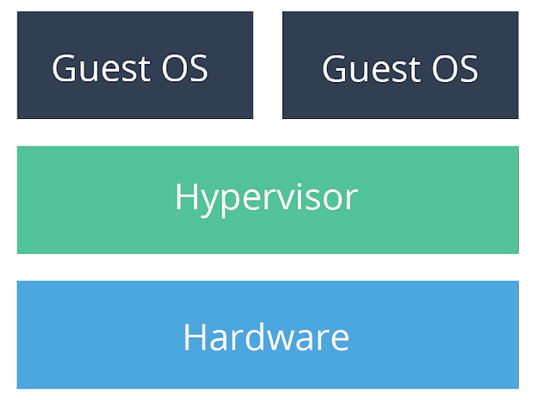
\includegraphics[width=0.7\linewidth]{images/Technologies/type_1_hypervisor.png}
	\caption{Type 1 (or bare metal) hypervisor architecture \cite{HypervisorsArchitectures}.}
	\label{fig:type_1_hypervisor}
\end{figure}

The greatest benefits of hypervisors are their robustness and scalability, enabling the efficient virtualization of large-scale applications and services.
However, the choice of creating a virtual machine using the Hyper-V Console Manager was dictated by two other reasons:

\begin{itemize}
	\item 
		The setup instructions described on the ebpf-for-windows GitHub repository tell the user to install a Windows virtual machine;
	\item 
		The so created isolated Windows 11 development environment provided a controlled space for testing and optimizing eBPF programs on the Windows platform.
		In fact, if anything goes wrong in this environment, we can just delete the virtual machine and create a new one, while if something bad happens on our host machine, we could break our computer.
\end{itemize}

So, to install eBPF on Windows the first thing that we have to do is to install our virtual machine.
To do so, we have to follow the instructions reported in the \textit{vm-setup.md} document \cite{WinVMSetupDoc}.
Besides the fact that that the virtual machine was configured with adequate resources to support development tasks effectively, the only thing worth noting is that during the quick creation of the virtual machine the option of ``Windows 11 dev environment'' is the only one that can be selected since our host computer has Windows 11 as operative system (the tutorial tells to choose the ``Windows 10 dev environment'' probably because at the time of writing of this document version 10 of Windows was the highest available, but Windows 11 works as well).  

After the ``one-time setup'' procedure is done, we have to decide how we are going to debug our virtual machine.
After a careful analysis of the requirements needed to install eBPF we decided to configure a kernel debugging connection over IP address.
In fact, since the eBPF for Windows binaries are not yet signed by Microsoft, they will only work on a machine with a kernel debugger attached and running or test signing is enabled.
Between the two, we decided to took the first route because it seemed easier.
To do so there are a few articles on the Microsoft Learn website, under the documentation section, that we have (once again) to follow by heart.
The two things that are worthy of note with this approach are the following:

\begin{itemize}
	\item 
		On our host computer we have to install a set of debugging tools for Windows.
		There are a few available \cite{DbgToolsWin}, but we decided to stick with the classic \textit{WinDbg}, a debugger that can be used to analyze crash dumps, debug live user-mode and kernel-mode code, and examine CPU registers and memory \cite{InstallWinDbg}.
		After following the installation path of this tool, we will find it under \colorbox{backcolour}{\lstinline[style=highlight]|$C:\\Program Files (x86)\\Windows Kits\\10\\Debuggers\\x64|};
	\item 
		Since it is very likely that sometimes we will shut down our virtual machine, every time that we are going to turn it on we have to start the kernel debugger attached to it (we will present later how to do it).
		This is quite inconvenient due to the fact that it requires a bit of time every time.  
\end{itemize}

At this point we have all the components that we will need on our host computer.
Now we have to install a series of applications on the virtual machine: under the \textit{Prerequisites} of \textit{Building eBPF for Windows} in the \textit{GettingStarted.md} document there is a list of things to install in order to build the repository project \cite{GetStartDoc}.
Moreover, to make WinDbg work and debug the virtual machine over IP, we have to install \textit{KDNET}, a debugging feature in Windows that allows remote kernel debugging over a network connection.

Once we have installed all the required tools, we are ready to start debugging our virtual machine.
With KDNET we have to set up the target machine (the one we want to debug) and the host machine (the one we will use for debugging) to communicate and then we can start the debugging session: an article on the Microsoft Learn websites tells us what to do \cite{SetUpNetDebug}.
However, even after we have followed all the listed steps the first time, whenever we want to turn on our virtual machine to work with eBPF, we have to redo some of these steps.
In particular, we have to:

\begin{itemize}
	\item 
		Open a \textit{Command prompt} with administrator privileges on both the machines;
	\item 
		Check the host IP address with the command \colorbox{backcolour}{\lstinline[style=commandline, language=bash]|ipconfig|} because if we let the \textit{Dynamic Host Configuration Protocol} (\textit{DHCP}, a network management protocol used on IP networks for automatically assigning IP addresses and other communication parameters to devices connected to the network using a client–server architecture) to assign automatically an IP address to our computer the address may vary;
	\item 
		On the virtual machine, in the \colorbox{backcolour}{\lstinline[style=commandline, language=bash]|C:\\KDNET|} folder (that we should have created if we followed the last mentioned article) we have to run \colorbox{backcolour}{\lstinline[style=commandline, language=bash]|C:kdnet <YourIPAddress> <YourDebugPort>|}, where the debug port must be within the range 50000-50039.
		This command will give us another command that we have to copy and run on the host machine.
		It will look like this: \colorbox{backcolour}{\lstinline[style=commandline, language=bash]|windbg -k net:port=<YourDebugPort>,key=<YourKey>|}, where the key consists of four alphanumeric strings separated by three dots;
	\item 
		On our host machine we have to:
		\begin{itemize}
			\item 
				Go to the folder where wh have installed WinDbg, which is \colorbox{backcolour}{\lstinline[style=commandline, language=bash]|"C:\\Program Files (x86)\\Windows Kits\\10\\Debuggers\\x64"|};
			\item 
				Run the command that we have copied from the virtual machine.
		\end{itemize}
		After we have run the command, WinDbg will start on our host machine.
		However, for now, it says ``Debuggee not connected''.
		We have to do a couple more steps to make it work;
	\item 
		Disable \textit{Enhanced session} on the virtual machine using the \textit{View} pull down menu in the VM;
	\item 
		Restart the virtual machine with the command \colorbox{backcolour}{\lstinline[style=commandline, language=bash]|shutdown -r -t|}.
		If after we restart the virtual machine one time the ``Debuggee not connected'' string did not change, we have to restart it a second time.
		If we do so, we should be able to see ``Debugger is running...''.
\end{itemize}

After everything is done we now have started our virtual machine with a kernel debugger attached.
In Figure \ref{fig:WinDbg} we can look at what we should see once we start the Windows debugger on our host machine.
In particular, Figure \ref{fig:WinDbgNc} shows the debugger interface when we run the command on our host machine, while Figure \ref{fig:WinDbgR} displays the interface once we reboot our virtual machine two times.

\begin{figure}[h]
	\centering
	\begin{subfigure}{.5\textwidth}
		\centering
		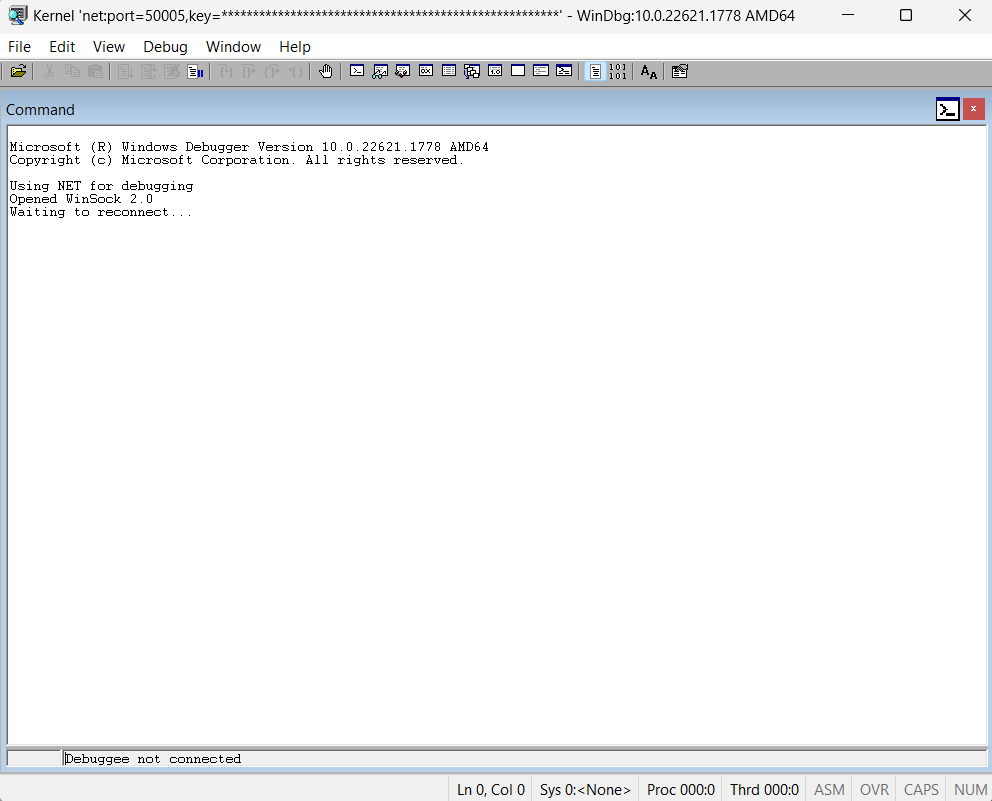
\includegraphics[width=0.7\linewidth]{images/WindowsDevelopment/WinDbg_nc.png}
		\caption{}
		\label{fig:WinDbgNc}
	\end{subfigure}%
	\begin{subfigure}{.5\textwidth}
		\centering
		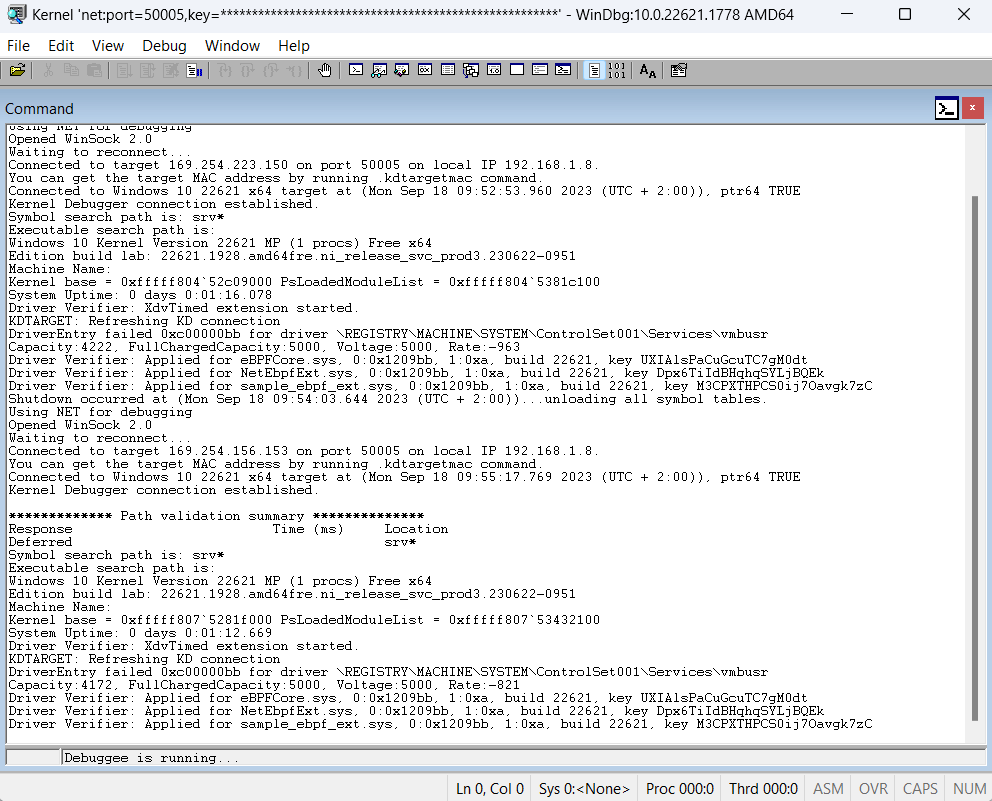
\includegraphics[width=0.7\linewidth]{images/WindowsDevelopment/WinDbg_r.png}
		\caption{}
		\label{fig:WinDbgR}
	\end{subfigure}	
	\caption{Windows debugger interface: (a) after starting WinDbg on our host machine; (b) after rebooting the virtual machine twice.}
	\label{fig:WinDbg}
\end{figure}

Note that this process must be done every time we want to turn on the virtual machine to work with eBPF.
Even if the IP address of you computer of the debug port change, the command that we have to run to start WinDbg on our host machine will always be the some.
However, if we do not do the kdnet procedure on our virtual machine, the debugger will never get attached to it.

At this point, remember to do the last point on the \textit{vm-setup.md} document which is \textit{Enable Driver Verifier on eBPF drivers}.

The last step that we have to make is to install ebpf-for-windows.
To do so, we have to follow the instructions given by the \textit{InstallEbpf.md} document \cite{InseBPFDoc}.
The easiest way to install eBPF into a test virtual machine is to stick to the so called ``Method 1''.
For this thesis we worked with the \textit{v0.9.0} version, but at the time of writing versions \textit{v0.10.0} and \textit{v0.11.0} were released.
We can understand how fast this technology is evolving on Windows.

Once we have done with all the set up part, we can now start developing some examples using the ebpf-for-windows project.
We must point out that from now on we will assume that we are working on a virtual machine that has been turned on with a kernel debugger attached, as we explained previously.

\section{ebpf for Windows}

To develop eBPF applications on Linux we used two projects that made this task relatively simple once we understood the logic behind eBPF.
Unfortunately, with ebpf-for-windows this doesn't happen.
However, the repository provides several documents in which it explains how to develop simple initial programs and how to debug them.

But before diving into that, we have to build our project: to do so, we have to follow the ``How to clone and build the project using Visual Studio'' section in the \textit{GettingStarted.md} document which consists of some operations besides cloning the repository.
After a series of attempt, we suggest to build the project by following the instructions given for ``Developer Command Prompt for VS 2022'' because we could not figure out how to perform this task with ``Visual Studio IDE'' since it says that there are some issues during the process.
After a few minutes, the process comes to an end and we have successfully built the project (there would probably be some warnings, but we can ignore them).

Now, we can finally start writing some eBPF programs.
We warmly invite the users new to eBPF on Windows (even the ones with plenty of experience with eBPF on Linux) to do the basic tutorial that can be found in the \textit{tutorial.md} document \cite{TutDoc}.
The complexity of the programs is really low, but the examples are very useful for understanding the outputs of a series of terminal commands regarding eBPF which in turn explain the programs' structure.

Even though the tutorial is pretty clear, we have to point out a few things to give a full perspective of writing an eBPF program on Windows:

\begin{itemize}
	\item 
		To explain how sections work, the tutorial first uses \colorbox{backcolour}{\lstinline[style=cstyle, language=C]|#pragma clang section|} and then switches to the macro \colorbox{backcolour}{\lstinline[style=cstyle, language=C]|SEC("...")|}.
		They have the same effect, but we suggest to stick to the traditional way that we already saw in Linux; 
	\item 
		From the tutorial we could see that inside the \colorbox{backcolour}{\lstinline[style=cstyle, language=C]|SEC("...")|} macro we could write anything we want.
		However, the number of hook points is limited (and they are different from Linux).
		To see what are the strings that can be written inside the macro to designate which hook point the eBPF program is designed for, we have to run \colorbox{backcolour}{\lstinline[style=commandline, language=bash]|ls HKCU:\\Software\\eBPF\\Providers\\SectionData|} on ``Windows PowerShell'' (not ``Command Prompt'') terminal with administrator privileges;
	\item 
		Among all the examples provided by the tutorial, not all of them can be installed inside the Windows kernel.
		If we want to do so, inside the \colorbox{backcolour}{\lstinline[style=cstyle, language=C]|SEC("...")|} macro we must use a string for a valid hook point;
	\item 
		If we have to include some header files, after we compile the program we could get an error that says that the file has not been found.
		To solve this we have to include the full path to that file (for example, to include \colorbox{backcolour}{\lstinline[style=commandline, language=bash]|bpf_helpers.h|} in our programs, we have to write \colorbox{backcolour}{\lstinline[style=commandline, language=bash]|C:\\eBPF-for-Windows.0.9.0\\build\\native\\include\\bpf_helpers.h|}.
\end{itemize}

Once we are done with the basic tutorial, there is a more complex one that illustrates how to understand and debug eBPF verification failures in the \textit{debugging.md} document \cite{DebugDoc}.
We are not going to cover it since our focus is to take the developed programs, install them inside the kernel, make them run and read some output strings.

\subsection{Making things work}

In the tutorial that we have done, under the section "Installing eBPF programs" it is explained how to load and unload an eBPF program in the kernel.
For practical reasons we are going to do this process using (once again) a simple ``Hello World!''-like program.

In Windows we have just to define the code of the program that we are going to inject in the kernel: we will call our program \colorbox{backcolour}{\lstinline[style=commandline, language=bash]|helloworld.c|}.

However, once we try to write some code (for example using Visual Studio), in our kernel debugger on our host machine several error messages will appear:

\begin{lstlisting}[style=commandline, language=bash, caption={Kernel debugger error messages}]
	WER/CrashAPI:2693: ERROR Invalid args, too  big block
	WER/CrashAPI:2882: ERROR PEB is not initialized
\end{lstlisting}

We can just ignore them: we will see later that our debugger works.
In the following there is the code of our \colorbox{backcolour}{\lstinline[style=commandline, language=bash]|helloworld.c|} program.

\begin{lstlisting}[style=cstyle, language=C, caption={``Hello world!'' kernel side program on Windows}, title=helloworld.c]
	#include "C:\\eBPF-for-Windows.0.9.0\\build\\native\\include\\bpf_helpers.h|"
	
	SEC("xdp")
	int print_helloworld(xdp_md_t *ctx) {
		int n = bpf_get_prandom_u32();
		bpf_printk("Hello World %d!", n);
		return 0;
	}
\end{lstlisting}

Looking at the code, there are a few things that we have to point at because they are different from Linux:

\begin{itemize}
	\item 
		There is no need to define a \colorbox{backcolour}{\lstinline[style=commandline, language=bash]|LICENSE|} for our BPF code;
	\item 
		As we mentioned earlier, we can now see that to include an header file for working with eBPF we have to include all the path to that file;
	\item 
		For this simple example we wanted to use two of the helpers provided for Windows.
		The full documentation about eBPF for Windows can be found on GitHub \cite{eBPFWinDoc}.
	\item 
		We decided to use the \colorbox{backcolour}{\lstinline[style=cstyle, language=C]|xdp|} hook point which defines a section meant as an XDP layer program.
		In other words, every time network packets are exchanged (for example, by searching something on the browser), the program is triggered.
\end{itemize}

The logic of the program is very simple: it gets a random integer from \colorbox{backcolour}{\lstinline[style=cstyle, language=C]|bpf_get_prandom_u32()|} and prints a string with \colorbox{backcolour}{\lstinline[style=cstyle, language=C]|bpf_printk()|}.
If we had tried to do like we did in Linux (i.e. defining a string and printing it), the program would fail the process of compilation because, as the time of writing, \colorbox{backcolour}{\lstinline[style=cstyle, language=C]|bpf_printk()|} can just print the standard string given as first parameter and from zero to a maximum of three integers.

Once we have written our program we are ready to inject it into the kernel.
To do so, we have to work from ``Command prompt'' with administrator privileges.
As we learned from the \textit{tutorial.md} document, first we have to compile our program with Clang:

\begin{lstlisting}[style=commandline, language=bash, caption={``Hello world!'' compile command}]
	clang -target bpf -Werror -g -O2 -c helloworld.c -o helloworld.o
\end{lstlisting}

We will not cover all the possible commands that the tutorial presented.
The curious users can look deeper into the characteristics of this program using the other commands.

Then we have to install this program into the kernel 

\begin{lstlisting}[style=commandline, language=bash, caption={``Hello world!'' installation command}]
	netsh ebpf add program helloworld.o
\end{lstlisting}

If the loading of the program into the kernel is successful we will get in return a program ID associated to it.
However, we have to mention a major problem that we faced when we were loading programs into the kernel.
To perform network debugging we have to create a \textit{virtual network adapter} (\textit{vNIC}) to emulate the behavior of a physical network adapter in order to provide network connectivity to our virtual machine.
However, since we are loading a program which has \colorbox{backcolour}{\lstinline[style=cstyle, language=C]|xdp|} as hook point, our virtual machine loses network connectivity.
This will also happen with all the other hook points that are shown on the repository since they are all related to networking: in fact, as the time of writing Windows does not provide many hook points (for example, there is no \colorbox{backcolour}{\lstinline[style=commandline, language=bash]|execve|} hook point like in Linux) and the ones available are not well-documented.
Inside the \textit{Settings} of our virtual machine we will display the following message:

\begin{lstlisting}[style=highlight, language=bash, caption={Network adapter problem}]
	You're connected using a virtual network adapter that we can't test.
\end{lstlisting}

This means that we could not browse in the internet in our virtual machine.
However, we will be able to watch debug messages anyway (but we could not figure out why).

Once the program is injected into the kernel, we are now ready to see some output strings.
In the \textit{GettingStarted.md} document, under the section ``Using tracing'', there is an explanation on how we can look at some debugging output.
eBPF on Windows uses \textit{Event Tracing for Windows} for logging traces: to view traces in real-time, the  \colorbox{backcolour}{\lstinline[style=commandline, language=bash]|tracelog.exe|} and \colorbox{backcolour}{\lstinline[style=commandline, language=bash]|tracefmt.exe|} commands from the \textit{Windows Driver Kit} (\textit{WDK}, a set of software tools from Microsoft that enables the development of device drivers for the Microsoft Windows platform that we are told to install in the In the \textit{Prerequisites} section of \textit{Building eBPF for Windows} in the \textit{GettingStarted.md} document) can be used.  
However, there is another very interesting way to do so, depending on where we want to generate our output.

If we want to see our debug strings in the ``Command prompt'' in real time we have to follow the instruction on the document mentioned above.
In particular, in another ``Command prompt'', we have to type in the following commands:

\begin{lstlisting}[style=commandline, language=bash, caption={tracelog real time debugging command}]
	cd C:\\Program Files (x86)\\Windows Kits\\10\\bin\\10.0.22621.0\\x64
	tracelog -start MyTrace -guid "%ProgramFiles%\[eBPF for Windows install folder]\ebpf-printk.guid" -rt 
	tracefmt -rt MyTrace -displayonly -jsonMeta 0
	tracelog -stop MyTrace
\end{lstlisting}

This is an important part of this process, so we have to be very careful about it:

\begin{itemize}
	\item 
		The first command brings in a folder where we can find the \colorbox{backcolour}{\lstinline[style=commandline, language=bash]|tracelog|} program which we installed as a prerequisite together with the \textit{Windows Driver Kit} and we are going to use to print our debug output;
	\item 
		The second command creates the trace session.
		instead of \colorbox{backcolour}{\lstinline[style=commandline, language=bash]|[eBPF for Windows install folder]|} we had to put our path to that folder: since it was located in \colorbox{backcolour}{\lstinline[style=commandline, language=bash]|C:\\Program Files\\ebpf-for-windows|}, we just had to replace the string between brackets with \colorbox{backcolour}{\lstinline[style=cstyle, language=C]|ebpf-for-windows|}.
		Moreover, we just want to look at the output printed by \colorbox{backcolour}{\lstinline[style=cstyle, language=C]|bpf_printk()|}, so we specified the \colorbox{backcolour}{\lstinline[style=commandline, language=bash]|ebpf-printk.guid|} file in the command.
		However, we could look at all sort of messages if we replace it with \colorbox{backcolour}{\lstinline[style=commandline, language=bash]|ebpf-all.guid|}
	\item 
		The third command lets us view the tracing session in real time on terminal;
	\item 
		The last command closes the trace session.
\end{itemize}

After running the first three commands, every time that the program triggers, we will get a new string on our ``Command prompt'' every time the program is triggered that should look like this:

\begin{lstlisting}[style=commandline, language=bash, caption={tracelog real time message output}]
	[CPU_ID]process_ID.thread_ID::gg/mm/yyyy-hh:mm:ss.sss [EbpfForWindowsProvider]{"Message":"Hello World x!"}
\end{lstlisting}

Apart from the IDs (the CPU one is just a number, while the process and the thread ones are in hexadecimal) and the date and time information, at the end we get our debugging message (\colorbox{backcolour}{\lstinline[style=cstyle, language=C]|x|} is the number generated randomly which varies in each message).
Once we are done with the tracing session, we press \colorbox{backcolour}{\lstinline[style=commandline, language=bash]|CTRL+C|} to interrupt the execution fo the \colorbox{backcolour}{\lstinline[style=commandline, language=bash]|tracefmt|} command and then we execute the fourth command of the ones previously shown.
Then, we run the last command to stop the tracing session: if we do not do this, we will not be able to start a new tracing session with the \colorbox{backcolour}{\lstinline[style=commandline, language=bash]|tracelog|} command.

However, once we close our terminal, all the information that we got from our tracing session gets lost.
On Windows there is a way to save all the debug messages in a file (and this could not be done on Linux).
The process is similar to before, but this time the command that we have to run are the following:

\begin{lstlisting}[style=commandline, language=bash, caption={tracelog kernel debugging commands}]
	cd C:\\Program Files (x86)\\Windows Kits\\10\\bin\\10.0.22621.0\\x64
	tracelog -start MyTrace -guid "%ProgramFiles%\[eBPF for Windows install folder]\ebpf-printk.guid" -kd
	tracelog -stop MyTrace
	netsh trace convert LogFile.Etl Output.csv csv
\end{lstlisting}

There are a few important things to look at:

\begin{itemize}
	\item 
		The first command is the same as before;
	\item 
		The second command does the same thing as before, but it has \colorbox{backcolour}{\lstinline[style=cstyle, language=C]|-kd|} instead of \colorbox{backcolour}{\lstinline[style=cstyle, language=C]|-rt|} at its end: this changes everything.
		In fact, now we can see the output messages in two different places:
		\begin{itemize}
			\item 
				In the kernel debugger interface;
			\item 
				In a \colorbox{backcolour}{\lstinline[style=cstyle, language=C]|LogFile.Etl|} which can be found in the same directory as \colorbox{backcolour}{\lstinline[style=cstyle, language=C]|tracelog|} (i.e. \colorbox{backcolour}{\lstinline[style=cstyle, language=C]|C:\\Program Files (x86)\\Windows Kits\\10\\bin\\10.0.22621.0\\x64|}).
		\end{itemize}
		Now, every time the program gets triggered, the kernel debugger interface prints a new message and the \colorbox{backcolour}{\lstinline[style=cstyle, language=C]|LogFile.Etl|} gets updated.
		It is a bit like before where in ``Command prompt'' new debug messages were printed in real time, but now they are printed in different locations;
	\item 
		The third command works in the same way as before;
	\item 
		The last command is a new one and we used it to transform the \colorbox{backcolour}{\lstinline[style=cstyle, language=C]|Etl|} file generated by \colorbox{backcolour}{\lstinline[style=cstyle, language=C]|tracelog|} in a \colorbox{backcolour}{\lstinline[style=cstyle, language=C]|csv|} file to make it readable.
		This file has as many rows as the number of messages that were printed by our program and quite a few columns which contain different information about our messages and we can find it in the same directory of the \colorbox{backcolour}{\lstinline[style=cstyle, language=C]|Etl|} file.
\end{itemize}

In the kernel debugger interface the printed messages have a very similar structure as the ones printed in ``Command prompt'' with the previous sequence of commands:

\begin{lstlisting}[style=commandline, language=bash, caption={tracelog kernel debugging message output}]
	[CPU_ID]process_ID.thread_ID::gg/mm/yyyy-hh:mm:ss.sss [EbpfForWindowsProvider/EbpfGenericMessage]{"Message":"Hello World x!"}
\end{lstlisting}

In addition we have the information about the event name which, in this case, is \colorbox{backcolour}{\lstinline[style=cstyle, language=C]|EbpfGenericMessage|}.

Instead, in the \colorbox{backcolour}{\lstinline[style=cstyle, language=C]|csv|} file all the information is disposed into columns: we can find the event name, the process ID, the date and time, the user data which contains just our \colorbox{backcolour}{\lstinline[style=cstyle, language=C]|Hello World x!|} message and many more. 

These are two ways to perform debugging with \colorbox{backcolour}{\lstinline[style=cstyle, language=C]|bpf_printk()|} on Windows.
Once we are done with the tracing session, we must remember to remove the program from where we have installed it with the following command:

\begin{lstlisting}[style=commandline, language=bash, caption={``Hello world!'' delete command}]
	netsh ebpf delete program program_id
\end{lstlisting}

In this case, the \colorbox{backcolour}{\lstinline[style=cstyle, language=C]|program_id|} is the one that we get in return when we installed the program.

\section{windows ebpf starter}

At this point we have understood how to work with eBPF on Windows.
However, we can clearly see that the procedure that we have to do every time to get some information about our program is quite long and complex.
If we make a comparison between what the projects that we have seen in Linux (i.e. BumbleBee and libbpf-bootstrap) and ebpf-for-windows, the second loses due to the difficulty of use.

Luckily, during our research, we came across an article written in a blog of an Indian IT company founded in 2020 that works on security for distributed devices and data called \textit{Subconscious Compute}.
In this article, published at the beginning of 2023, the author Gurnoor Virdi, who made an internship with them, talks about eBPF programming on Windows \cite{eBPFWinSubComBlogArticle}: he covers the topics of installation and programming model of eBPF (which we already discussed in the previous paragraph) and, most importantly for us, talks about an environment that, after a first reading, looks similar to libbpf-bootstrap.

However, the virtual machine setup and the installation of the eBPF runtime (what we get after we follow the ``Method 1'' in the \textit{InstallEbpf.md} document of the ebpf-for-windows repository) have to be performed anyway if we want to run an eBPF program.
So, once again we will take for granted that the virtual machine has been turned on with a kernel debugger attached.

Now that everything is set up we can start working on the environment described in the article.
Unfortunately, the repository that is mentioned in the document is on \textit{GitLab}, another open source web platform used to manage Git repositories, and only the Subconscious Compute users have access to it.
However, we wrote them an email asking if we could have had access to that repository and they replied saying that they would put the repository on GitHub and make it open source under AGPL license: the project is called \textit{windows-ebpf-starter} \cite{WineBPFStarterRepo}.

After we cloned the repository on our virtual machine, we built the environment by following the instructions on the article and did the tutorial about ``Writing and compiling a simple eBPF program''.
Once we became familiar with the environment, we decided to reproduce the same examples that we did in Linux to make a fair comparison between two programs that should do the same thing.
For this purpose, in the following we are going to present a program very similar to the one that used an \colorbox{backcolour}{\lstinline[style=cstyle, language=C]|HashMap|}: we will call it \colorbox{backcolour}{\lstinline[style=cstyle, language=C]|hash_map_use.c|}

\begin{lstlisting}[style=cstyle, language=C, caption={hash\_map\_use.c program using windows-ebpf-starter}, title=hash\_map\_use.c]
	#include "stdint.h"
	#include "bpf_helpers.h"
	#include "bpf_helper_defs.h"
	#include "ebpf_structs.h"
	
	SEC("maps")
	ebpf_map_definition_in_file_t hash_map = {
		.type = BPF_MAP_TYPE_HASH,
		.max_entries = 256 * 1024,
		.key_size = sizeof(uint64_t),
		.value_size = sizeof(int64_t),
	};
	
	static void hash_map_use(uint64_t pid, uint64_t time_stamp){
		bpf_printk("### BEGIN HASH MAP USE ###");
		
		int64_t update;
		int64_t delete;
		
		uint64_t *found;
		uint64_t *deleted;
		
		update = bpf_map_update_elem(&hash_map, &pid, &time_stamp, EBPF_ANY);
		
		bpf_printk("UPDATE: pid %d - update %d.", pid, update);
		
		bpf_printk("key pid %d - ts %llu - update %d.", pid, time_stamp, update);
		
		found = (uint64_t *) bpf_map_lookup_elem(&hash_map, &pid);
		
		if (found) {
			bpf_printk("FOUND IN HASH MAP: pid %d - *found %llu.", pid, *found);
		} else {
			bpf_printk("NOT FOUND IN HASH MAP");
		}
		
		delete = bpf_map_delete_elem(&hash_map, &pid);
		
		bpf_printk("DELETE: pid %d - delete %lld.", pid, delete);
		
		deleted = (uint64_t *)bpf_map_lookup_elem(&hash_map, &pid);
		
		if (deleted) {
			bpf_printk("DELETED IN HASH MAP: pid %d - *deleted %llu).", pid, *deleted);
		} else {
			bpf_printk("NOT DELETED IN HASH MAP.");
		}
		
		bpf_printk("### END HASH MAP USE ###\n\n");
	}
	
	SEC("xdp")
	int print_pid_hash_map(xdp_md_t* ctx)
	{
		uint64_t pid;
		uint64_t time_stamp;
		
		pid = bpf_get_current_pid_tgid() >> 32;
		time_stamp = bpf_ktime_get_ns(); 
		
		bpf_printk("BPF triggered from PID %d at time %llu.\n", pid, time_stamp);
		
		hash_map_use(pid, time_stamp);
		
		return 0;
	}
\end{lstlisting}

Apart from the different way of defining an eBPF map and some types of some variables, the logic of the program is the same as the program in Linux: 

\begin{itemize}
	\item 
		take the process ID with \colorbox{backcolour}{\lstinline[style=cstyle, language=C]|bpf_get_current_pid_tgid() >>32|} and the time from system boot with \colorbox{backcolour}{\lstinline[style=cstyle, language=C]|bpf_ktime_get_ns()|};
	\item 
		Add them to the \colorbox{backcolour}{\lstinline[style=cstyle, language=C]|HashMap|} with the \colorbox{backcolour}{\lstinline[style=cstyle, language=C]|pid|} as key and the \colorbox{backcolour}{\lstinline[style=cstyle, language=C]|time_stamp|} as value;
	\item 
		Look for the \colorbox{backcolour}{\lstinline[style=cstyle, language=C]|pid|} value in the map (which will always be found);
	\item 
		Delete the \colorbox{backcolour}{\lstinline[style=cstyle, language=C]|pid|}-\colorbox{backcolour}{\lstinline[style=cstyle, language=C]|time_stamp|} couple from the map;
	\item 
		Check if the delete operation has been done successfully.
\end{itemize}

Once we compile the program with the \colorbox{backcolour}{\lstinline[style=commandline, language=bash]|build.bat|} file provided by the project, we can then load it into the kernel and start a tracing session with the same procedure as we saw earlier.

After doing so, we will see the following output:

\begin{lstlisting}[style=commandline, language=bash, caption={hash\_map\_use.c program output}]
	"BPF triggered from PID ``pid'' at time ``time_stamp''."
	"### BEGIN HASH MAP USE ###"
	"UPDATE: pid ``pid'' - update 0."
	"key pid ``pid'' - ts ``time_stamp'' - update 0."
	"FOUND IN HASH MAP: pid ``pid'' - *found ``time_stamp''."
	"DELETE: pid ``pid'' - delete 0."
	"NOT DELETED IN HASH MAP."
	"### END HASH MAP USE ###"
\end{lstlisting}

There are a few interesting things about this output messages:

\begin{itemize}
	\item 
		We did report just the debug messages, omitting the information about the process and thread IDs, the date and time and the CPU number;
	\item 
		As the output of the Linux program, \colorbox{backcolour}{\lstinline[style=cstyle, language=C]|pid|} and \colorbox{backcolour}{\lstinline[style=cstyle, language=C]|time_stamp|} are between quotes because they depend on the particular trigger of the program;
	\item 
		Due to the problem with the virtual network adapter that we have discussed previously, the process ID will always be 0, meaning that the system is in idle.
		However, this is not important if we just want to show how this program works;
	\item 
		The second-to-last message suggests that the delete operation has not been performed successfully, even though the \colorbox{backcolour}{\lstinline[style=cstyle, language=C]|bpf_map_delete_elem()|} returns 0.
		We could not figure out why this happens.
		We tried to develop the exact same program using an \colorbox{backcolour}{\lstinline[style=highlight, language=bash]|ArrayMap|} instead of the \colorbox{backcolour}{\lstinline[style=highlight, language=bash]|HashMap|} and all the debug messages are the same except for the penultimate one, which is \colorbox{backcolour}{\lstinline[style=highlight, language=bash]|"DELETED IN ARRAY: pid ``pid'' - *deleted 0."|}.
		It looks like that the delete method works well with the \colorbox{backcolour}{\lstinline[style=highlight, language=bash]|ArrayMap|}, but gives some problems with the \colorbox{backcolour}{\lstinline[style=highlight, language=bash]|HashMap|};
	\item 
		We remember that with \colorbox{backcolour}{\lstinline[style=cstyle, language=C]|bpf_printk()|} we can just print numbers on Windows, so we could not print the \colorbox{backcolour}{\lstinline[style=highlight, language=bash]|deleted|} pointer to see its value.
\end{itemize}

Besides learning some new things about eBPF maps, it seems that this project, which we looked at with hope, does not significantly simplify things when we have to load a program inside the kernel and look at some debug output.
It make the process of compilation easier because it defines the \colorbox{backcolour}{\lstinline[style=commandline, language=bash]|build.bat|} file which allows us to compile multiple programs at once, but other than that we have to use again the commands that are shown in the \textit{tutorial.md} document in the ebpf-for-windows repository.

However, the article of Gurnoor Virdi does not stop with the writing of some simple eBPF programs: the section called ``Working with userspace'' is the most interesting part about this project because it shows how we can manage the lifetime of an eBPF program through an user space application (like we did with libbpf-bootstrap).

The idea is the same of the one that we have already seen in Linux: create a user space application that uses a series of methods to manage the various phases that an eBPF kernel side program goes through: opening, loading, attaching and unloading.
However, these methods are not generated automatically in a skeleton file by the environment after we compile the kernel source code of the program that we want to control from user space: they are defined in an header file inside the eBPF runtime called \colorbox{backcolour}{\lstinline[style=commandline, language=bash]|libbpf.h|} under the folder
\colorbox{backcolour}{\lstinline[style=commandline, language=bash]|..\\ebpf-for-windows.0.9.0\\build\\native\\include\\libbpf\\src|} (the documentation of this header can be found in a page of the eBPF for Windows documentation on GitHub \cite{eBPFWinlibbpfHeader}).
In fact, we only need two things to make the user space application work:

\begin{itemize}
	\item 
		The path to the object file \colorbox{backcolour}{\lstinline[style=commandline, language=bash]|.o|} generated from the kernel source code after the process of compilation;
	\item 
		The name of the eBPF program that we want to load into the kernel (in other words it is the name of the function defined after \colorbox{backcolour}{\lstinline[style=cstyle, language=C]|SEC("hook_point")|}).
\end{itemize}

Once we have these 2 things we can use the \colorbox{backcolour}{\lstinline[style=cstyle, language=C]|bpf_object__open()|} method to create a pointer to a \colorbox{backcolour}{\lstinline[style=cstyle, language=C]|bpf_object|} which we are going to use in the following phases with other self-explanatory methods, such as \colorbox{backcolour}{\lstinline[style=cstyle, language=C]|bpf_object__load()|} to load the object code into the kernel, \colorbox{backcolour}{\lstinline[style=cstyle, language=C]|bpf_object__attach()|} to attach the program to an hook point and \colorbox{backcolour}{\lstinline[style=cstyle, language=C]|bpf_object__close()|} to unload the object code from the kernel.

However, we tried to do the tutorial presented in the article, but we could not manage to correctly compile the user space application.
Every time we get a fatal error saying that the  \colorbox{backcolour}{\lstinline[style=commandline, language=bash]|\#include|} files cannot be found.
In particular, we get the error code \colorbox{backcolour}{\lstinline[style=commandline, language=bash]|0x2|} which corresponds to \colorbox{backcolour}{\lstinline[style=commandline, language=bash]|ERROR_FILE_NOT_FOUND|}. 
This error code indicates that the system or a program attempted to perform an operation on a file or directory that does not exist at the specified location.

We get this error for including all the headers, but for different reasons:

\begin{itemize}
	\item 
		If we include a standard C library (such as \colorbox{backcolour}{\lstinline[style=commandline, language=bash]|iostream|}), the compiler says that it cannot find such file;
	\item 
		If we include an header file from the eBPF runtime (such as \colorbox{backcolour}{\lstinline[style=commandline, language=bash]|libbpf.h|}), even if we put the full path to that file the compiler says that he cannot find some other header.
		In fact, in the header files of the eBPF runtime there are plenty of \colorbox{backcolour}{\lstinline[style=commandline, language=bash]|\#include|} of some other headers.
\end{itemize}

We think that the problem is the way in which the project is structured: in the tutorial we are told to modify the \colorbox{backcolour}{\lstinline[style=commandline, language=bash]|Makefile|} and add our particular paths to the location of the include directory of the eBPF development files we downloaded through the \colorbox{backcolour}{\lstinline[style=commandline, language=bash]|nuget|} package, i.e. \colorbox{backcolour}{\lstinline[style=commandline, language=bash]|..\\ebpf-for-windows.0.9.0\\build\\native\\include|} and to the location of the lib directory containing \colorbox{backcolour}{\lstinline[style=commandline, language=bash]|EbpfApi.lib|} from the eBPF install directory. i.e. \colorbox{backcolour}{\lstinline[style=commandline, language=bash]|..\\ebpf-for-windows.0.9.0\\build\\native\\lib|}.
We think that this tells to the compiler to look for the files to include just in the first of these two folders, but, obviously, not all headers are in it.

So, although windows-ebof-starter looks very promising, we were only able to make it work with the kernel-side code and the commands that are reported in the \textit{tutorial.md} document in ebpf-for-windows.

